\chapter{信誉评估算法原型系统的实现}

本章对车辆信誉评估算法的原型系统进行了详细的介绍。该系统主要由浏览器端和智能合约端两部分构成。浏览器端主要进行车辆行驶数据获取、车辆交互模拟以及行驶状态的可视化展示,智能合约端负责数据的存储以及车辆信誉评估算法的具体实现。原型系统的整体架构如图~\ref{fig:proto}所示。

\begin{figure}
  \centering
  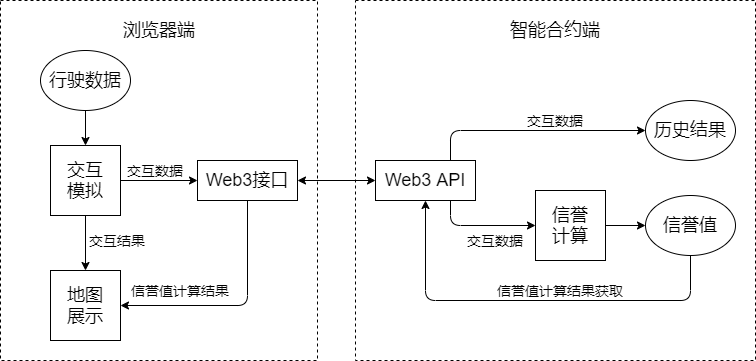
\includegraphics[width=0.8\linewidth]{figures/proto.png}
  \caption{车辆信誉评估原型系统架构图}
  \label{fig:proto}
\end{figure}

\section{总体框架及运行环境}
信誉评估算法的原型系统框架主要分为两个部分:浏览器端及智能合约端。浏览器端模拟实际场景中的车辆终端,进行位置信息获取、车辆交互等数据处理任务;智能合约端模拟实际场景中的路侧单元(RSU),对车辆的信誉进行更新和维护。考虑到智能合约对于复杂运算存在较大的限制,同时区块链上的大量计算需要付出相应的执行费用,因此该原型系统中位置验证、消息传播的模拟由浏览器端负责,将模拟的交互结果上传至区块链后,合约端仅负责信誉值的评估计算。本原型系统的运行流程如下:
\begin{enumerate}
    \item 系统初始化。浏览器端通过web3.js接口对信誉评估的智能合约进行初始化,同时加载地图和车辆行驶的道路数据,转化为Geohash格式存储,便于之后的合约计算。结合加载的缓存数据,为目标车辆生成用户的通用唯一识别码,作为该车辆身份的确认证明,此后浏览器端将对该目标车辆的行驶路线和信誉值变化进行追踪。
    \item 模拟车辆交互。车辆交互结果的模拟是浏览器端的重要部分,该步骤中程序对目标车辆和其行驶途中遇到的邻近车辆分别进行位置验证和消息传播的模拟,并最终给出模拟交互的结果。具体实现方式见3.2节。
    \item 上传交互结果。获得交互结果(位置验证结果或者邻近车辆给出的消息评价)之后,浏览器端利用web3.js接口将该结果的相关数据打包上传至区块链,在合约端进行结果数据的存储,并进行信誉值计算。
    \item 信誉评估。信誉评估是合约端程序的主要内容,依据模拟交互的结果、数据上传的时间及上一章中设计的算法进行信誉值的计算和更新。针对智能合约在计算开销方面的限制,笔者在信誉评估合约中采取了一系列简化计算的措施,具体情况见3.3节。
    \item 地图展示。浏览器端使用了leaflet(一个开源的JavaScript互动地图库,适用于移动设备)\cite{leaflet}进行地图及车辆行驶路线的展示。在合约端完成信誉值的更新之后,浏览器端可以通过web3.js接口获取更新之后的信誉值,该信誉值及本次车辆交互的结果都可以在leaflet地图中得到可视化展示,具体情况见3.4节。
\end{enumerate}

本章中的系统在Ubuntu 20.04操作系统中实现,使用Solidity v0.8.0实现智能合约,并通过Web3.js v1.2.9实现浏览器端功能,以及与以太坊区块链的对接。在系统开发及测试过程中,使用Truffle v5.1.62进行智能合约的编译与本地私有链的部署,同时结合私有链的可视化工具Ganache v6.12.2进行便利的调试与开发。

\section{车辆交互模拟}
该原型系统中,浏览器端负责车辆交互的模拟,其中包括位置验证的模拟和消息传播的模拟。对于位置验证,每次模拟只涉及到目标车辆和一台邻近车辆;对于消息传播,每次交互(即同一条消息的发送与评价)涉及到目标车辆及其周围的多方车辆。在程序中两种场景的模拟独立进行,分别选取对应的参与车辆并各自进行交互的模拟,两者的结果互不影响。下面,文章将分别介绍两种交互的具体模拟形式。
\subsection{位置验证模拟}
在目标车辆行驶过程中,它可以向一定范围内的邻近车辆发送请求,表明希望他人为自己提供位置验证,当一辆邻近车辆收到该请求后,可以视为两辆车进行了一次位置验证的交互,而最终是否获取有效的位置验证即为本次交互结果成功或失败的判断标准。在实际情况中,位置验证是否成功可能取决于以下因素:参与交互的车辆对当前行驶区域的熟悉程度;交互车辆获取地理位置信息的准确度;交互车辆之间的通讯信号强度;交互车辆中是否存在恶意行为。

在本文所实现的原型系统中,对位置验证过程中通信的具体内容不做过多考虑,仅通过上述影响因素模拟位置验证的结果,具体思路如下:
\begin{enumerate}
    \item 对于目标车辆当前所处区域(在该原型系统中,区域按照具体的城市道路进行划分),在每个区域中,根据目标车辆历史记录中对该区域的到访情况,即车辆对该区域的熟悉程度,该车辆拥有一个位置验证成功率的基准波动范围。目标车辆经常行驶的区域,对应的基准范围相对更高;对于不够熟悉或者未曾到访过的区域,对应的基准范围相对较低。
    \item 目标车辆与邻近车辆进行一次位置验证交互时,其成功率在上述基准范围之内波动,并最终由两辆车之间的交互距离所确定。其中,交互距离为两辆车在行驶途中所能达到的最短距离,该距离与位置验证的成功率成一次负相关关系。
    \item 在确定了当次位置验证的成功率之后,程序通过伪随机数模拟得到最终的位置验证结果为成功还是失败,并将该结果及相关数据上传至合约端。
    \item 特别地,在参数测试与评估阶段,为了有针对性地研究特定环境下各参数取值对应的特征,部分测试中略去了行驶道路和交互距离对验证成功率的影响,仅通过伪随机数模拟来观察在确定的验证成功率条件下,不同参数取值对系统的影响。
\end{enumerate}

\subsection{消息传播模拟}

在特定事件(比如道路拥堵、交通事故等)发生时,目标车辆可以向邻近车辆发送消息,告知自己观察到的事件信息。由于特殊事件的发生属于偶然情况,因此消息传播这一交互行为的频率相对较小,并且每次仅对一定范围内的特定车辆群体有效。邻近车辆对消息内容的评价和自身与实际事件发生位置之间的距离相关,在本系统中使用该车辆与目标车辆之间的距离进行替代。

与位置验证类似,在程序实现中笔者同样忽略具体的事件及消息内容,主要对接收消息的车辆群体及它们给出的消息反馈进行模拟,主要流程如下:
\begin{enumerate}
    \item 确定接收消息的邻近车辆。以目标车辆为中心,取与之相距在五个单位之内的所有车辆,为接收到本次交互消息并给出评价的车辆群体。在模拟测试中,周边车辆沿道路呈区域性的均匀分布(车辆密度不同);在实际测试中,周边车辆的分布则完全由真实数据决定。
    \item 模拟邻近车辆的消息评价。每台收到消息的车辆给出对消息的打分,分数是$[1,10]$之间的整数。在参数测试阶段,为了对距离衰减系数$\gamma$的取值进行评估,并对消息总评价进行可信区域划分,该部分选取了几种消息评价的分布情况,分别进行模拟:评价分数在$[1,10]$之间完全随机;与目标车辆距离较近的中心车辆给出的分数和边缘车辆相差较大(中心车辆评价大于5分、边缘车辆评价小于5分,或者相反情况)。
    \item 在浏览器端收集各邻近车辆给出的消息评分,并预先计算每辆车与目标车辆之间的距离,保证评分与交互距离一一对应,并将数据打包上传至合约端。
\end{enumerate}

\section{信誉评估智能合约}

智能合约中实现了第2章中的信誉评估算法,并进行相关数据的存储,在实际应用中对应路侧单元(RSU)的功能。由于合约部署在区块链上,具有公开透明、可追溯等特点,因此为信誉计算提供了安全性的保障,从底层结构上确保这一过程是具有权威性的,避免了对信誉值可能的篡改行为。

在本文实现的合约中,以用户为单位进行数据的维护,通过通用唯一识别码(UUID)与用户信息的数据结构user建立映射。在用户信息中,主要维护的数据内容包括历史数据提交时间、位置验证的历史结果统计、用户信誉值等。除此之外,合约中还实现了message数据结构,用于消息传播发生时的信誉计算,其中维护消息发送者UUID、各车辆给出的消息评分、各车辆与消息发送者之间的距离等。

当且仅当目标车辆与邻近车辆完成一次交互模拟之后,浏览器端会上传相应的数据并调用合约中信誉计算的相关接口;合约端则根据交互类型,选择进行位置验证或消息传播结果的数据处理,并进一步完成信誉值的更新。

由于智能合约端的每次计算都会消耗一定的gas(执行开销),同时对内存访问和复杂的数学函数都具有一定的限制,因此合约实现的难点之一就在于在原有算法的基础上对合约计算进行尽可能的简化,采用的具体措施包括:

\begin{enumerate}
    \item 使用Geohash存储地理位置信息。Geohash是一种地理编码系统,它将传统的经纬度位置信息转换为一维的字符串,每个字符串对应一块矩形的地理区域\cite{lwq}。使用这种方式存储位置信息,可以在精度允许的范围内对车辆进行定位,同时将与距离相关的计算过程和结果全部转移到整数范畴中,相比于利用经纬度计算得到了大幅度的精简。
    \item 在浏览器端进行数据预处理。为了节省合约端的计算开销,部分不与信誉值直接相关的数据可以在浏览器端提前进行计算,比如消息传播过程中各车与目标车辆之间的距离,而在合约端只保留信誉计算的核心步骤。
    \item 简化参数相关的计算过程。对于合约端较为复杂的计算步骤,可以事先计算出中间结果,将中间结果作为实际计算的参数。譬如消息传播中涉及到的指数计算,由于系统实现中$dis(i,j)$的实际取值仅限于$[0,5]$之间的整数,因此在参数$\gamma$确定后可直接计算得到几种可能的幂值并将其作为参数写入程序中,在信誉计算的过程中根据距离直接获取相应的中间值即可。
\end{enumerate}

\section{地图展示}
本章使用了OpenStreetMap(OSM)\cite{osm}提供的开源地图获取北京市的道路信息,并利用osm2pgrouting\cite{pg}转换工具提取出道路数据信息进行存储。在原型系统的浏览器端,本章使用leaflet地图组件加载离线OSM数据,并在地图上进行车辆行驶数据、友邻交互以及信誉评估结果的可视化展示。地图中的具体展示内容主要包括以下三项:
\begin{enumerate}
    \item 目标车辆的行驶轨迹。根据目标车辆提供的位置信息,浏览器端在地图上进行数据点的绘制,并最终构成一条完整的车辆行驶轨迹。
    \item 目标车辆与邻近车辆的交互结果。当浏览器端发生一次车辆间的模拟交互时,地图组件将绘制参与交互的邻近车辆此时所在的位置,并通过具体的数据点颜色体现本次交互的模拟结果。
    \item 目标车辆的实时信誉。在绘制目标车辆的行驶轨迹时,每个数据点的颜色代表了车辆此时对应的信誉值评估结果。浏览器端通过web3.js接口从合约端获取更新后的信誉值,并据此选择对应的中间梯度颜色绘制数据点。
\end{enumerate}
本文将在第5章中对地图展示的实际效果与表现含义做进一步的说明。

\section{本章小结}
本章介绍了车辆信誉评估算法原型系统的具体实现。该系统在浏览器端进行车辆交互的结果模拟以及行驶状态的可视化展示,在合约端完成数据存储以及车辆信誉评估算法的实现,通过区块链保证了信誉计算的安全性与可靠性。同时,为了解决智能合约对于复杂数学计算的限制,系统在合约编写方面对具体计算方式进行了一系列优化措施。